% Niveau :      PCSI *
% Discipline :  Chimie Orga I
% Mots clés :   Spectrométrie UV-visible, Réactions acidobasiques

\begin{exercise}{Chimie click, chimie verte}{2}{PCSI}
{Solvants}{bermu}



\begin{questions}
    \questioncours Différentes étapes de la solvatation d'un soluté dans un solvant. \\
    On illustrera la question d'exemple en rentrant dans le détail des différents types de solvants.

\begin{EnvUplevel}
Un des principes très importants de chimique organique est de réduire la quantité de solvants organiques utilisés.

Une des tendances actuelles en chimie de synthèse est la chimie click au micro-onde de la réaction de Biginelli :
\begin{center}
    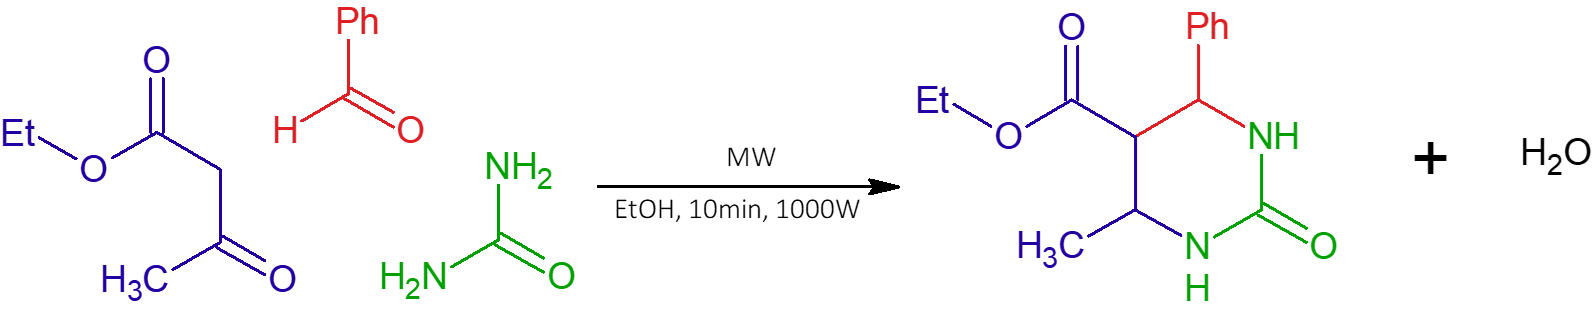
\includegraphics[width=.9\linewidth]{chimiePC/atomes/click.png}
\end{center}

\end{EnvUplevel}
    
    \question Classiquement, pour faire une telle réaction on utilise du toluène et un catalyseur qui sont tous deux très polluants.
    
    \begin{parts}
        \part Justifier le choix du toluène (solvant apolaire).
        
        \part \`A la suite de la réaction, il faut ensuite extraire le produit. Donner le principe de l'extraction par solvants et indiquer ici un solvant que l'on pourrait utiliser pour cela.
    
    \end{parts}
    
    \question En chimie click, on utilise uniquement de l'éthanol pour la réaction. Celle-ci est activée grace aux micro-ondes.
    
    \begin{parts}
        \part Justifier le choix de l'éthanol.
        
        \part Justifier que l'éthanol est excité par les micro-ondes et que cela permet de catalyser la réaction.
    \end{parts}
    
    \question Conclure quant aux gains écologique pour réaliser cette réaction. Pour information les 12 principes de la chimie verte ci-dessous.
    
    \begin{table}[H]
        \centering
        \begin{tabular}{ll}
            \\\hline\hline
            1. Prévention : moins de déchets ; &
            7. Matières renouvelables  ;\\
            2. Économie d'atomes : moins de sous-produits ; &
            8. Schéma de synthèse efficace ;\\
            3. Réactif doux : pas de substances toxiques ; &
            9. Catalyse ;\\
            4. Réduire la toxicité des produits utilisés ; &
            10. Produits biodégradables ;\\
            5. Pas de substances auxiliaires (solvants...) &
            11. Contrôle des conditions de réaction ; \\
            6. Conditions douces : CNTP ; &
            12. Réduire les risques d'accidents. \\ \hline
        \end{tabular}
        \caption{Principes de la chimie verte}
    \end{table}
    
    \question (\emph{Bilan}) Récapituler les rôles du solvant en chimie de synthèse et la manière de réduire son impact écologique.
\end{questions}
\end{exercise}